%%%%%%%%%%%%%%%%%%%%%%%%%%%%%%%%%%%%%%%%%%%%%%%%%%%%%%%%%%%%%%%%%%%%%%%%%%%%%
%%%
%%% File: utthesis2.doc, version 2.0jab, February 2002
%%%
%%% Based on: utthesis.doc, version 2.0, January 1995
%%% =============================================
%%% Copyright (c) 1995 by Dinesh Das.  All rights reserved.
%%% This file is free and can be modified or distributed as long as
%%% you meet the following conditions:
%%%
%%% (1) This copyright notice is kept intact on all modified copies.
%%% (2) If you modify this file, you MUST NOT use the original file name.
%%%
%%% This file contains a template that can be used with the package
%%% utthesis.sty and LaTeX2e to produce a thesis that meets the requirements
%%% of the Graduate School of The University of Texas at Austin.
%%%
%%% All of the commands defined by utthesis.sty have default values (see
%%% the file utthesis.sty for these values).  Thus, theoretically, you
%%% don't need to define values for any of them; you can run this file
%%% through LaTeX2e and produce an acceptable thesis, without any text.
%%% However, you probably want to set at least some of the macros (like
%%% \thesisauthor).  In that case, replace "..." with appropriate values,
%%% and uncomment the line (by removing the leading %'s).
%%%
%%%%%%%%%%%%%%%%%%%%%%%%%%%%%%%%%%%%%%%%%%%%%%%%%%%%%%%%%%%%%%%%%%%%%%%%%%%%%

\documentclass[11pt]{report}         %% LaTeX2e document.

%% Preamble starts here and goes until \begin{document}.

%% Special packages, kept (optionally) in their own directory for
%% general housekeeping purposes. Note that the path to the .sty
%% file must be specified if it is kept in a separate directory.
\usepackage{./packages/utthesis2}              
\usepackage{./packages/natbib}
\usepackage{./packages/gb4e}

%% Built-in packages
\usepackage{multicol} %% Multicolumnar support
\usepackage{graphicx} %% Support for \includegraphics with scale options

\newif\ifmasters		     %% Do not change
\newif\ifphd			     %% these lines.

 \mastersthesis   \masterstrue      %% Uncomment one of these lines.
% \phdthesis      \phdtrue           %% 


% \leftchapter                       %% Uncomment one of these if you want
 \centerchapter                     %% left-justified, centered or
% \rightchapter                      %% right-justified chapter headings.
                                     %% Chapter headings includes the
                                     %% Contents, Acknowledgments, Lists
                                     %% of Tables and Figures and the Vita.
                                     %% The default is \centerchapter.

% \singlespace                       %% Uncomment one of these if you want
\oneandhalfspace		     %% single-spacing, space-and-a-half
% \doublespace                       %% or double-spacing; the default is
                                     %% \oneandhalfspace, which is the
                                     %% minimum spacing accepted by the
                                     %% Graduate School.

%% Your official UT name.
\renewcommand{\thesisauthor}{(Insert your Official UT Name)}    

%% Your month of graduation.
\renewcommand{\thesismonth}{May}     

%% Your year of graduation.
\renewcommand{\thesisyear}{2013}      

%% The title of your thesis; use mixed-case.
\renewcommand{\thesistitle}{A Quick Guide to Starting your 
			    UT Thesis with \LaTeX}
				     
%% Your previous degrees, abbreviated; separate multiple degrees by commas.     
\renewcommand{\thesisauthorpreviousdegrees}{(list your previous degrees here)}
                                     
%% Your thesis supervisor; use mixed-case and don't use any titles or degrees.
 \renewcommand{\thesissupervisor}{Ada Lovelace}

\newif\ifcosuper                                     
%% Your PhD. thesis co-supervisor; if any. Use mixed case and don't use any 
%% titles or degrees. Uncomment if you have a co-supervisor. Do not change
%% \cosupertrue. (Ignored for Master's)
% \renewcommand{\thesiscosupervisor}{} \cosupertrue

%% Your remaining committee members. Only the first of these is used for
%% Master's theses/reports -- rest are applicable to Ph.D. only, ignored for
%% Master's
 \renewcommand{\thesiscommitteemembera}{James Bond}
 \renewcommand{\thesiscommitteememberb}{Professor 3}
 \renewcommand{\thesiscommitteememberc}{Professor 4}
 \renewcommand{\thesiscommitteememberd}{Professor 5}
% \renewcommand{\thesiscommitteemembere}{}
% \renewcommand{\thesiscommitteememberf}{}
% \renewcommand{\thesiscommitteememberg}{}

%% Your permanent address; use "\\" for linebreaks.
\renewcommand{\thesisauthoraddress}{}

%% Your dedication, if you have one; use "\\" for linebreaks.
\renewcommand{\thesisdedication}{Put your dedication here.}

%%%%%%%%%%%%%%%%%%%%%%%%%%%%%%%%%%%%%%%%%%%%%%%%%%%%%%%%%%%%%%%%%%%%%%%%%%%%%
%%%
%%% The following commands are all optional, but useful if your requirements
%%% are different from the default values in utthesis.sty.  To use them,
%%% simply uncomment them.


%\renewcommand{\thesiscommitteesize}{...}
%\renewcommand{\masterscommitteeminusone}{...} %% This line not needed for Ph.D.
				    %% Uncomment these only if your thesis
				    %% committee does NOT have 5 members
				    %% for \phdthesis or 2 for \mastersthesis.
				    %% Replace the "..." with the correct
				    %% number of members. 

% \renewcommand{\thesisdegree}{...}   
				    %% Uncomment this only if your thesis
				    %% degree is NOT "DOCTOR OF PHILOSOPHY"
				    %% for \phdthesis or "MASTER OF ARTS"
				    %% for \mastersthesis.  Provide the
				    %% correct FULL OFFICIAL name of
				    %% the degree.

% \renewcommand{\thesisdegreeabbreviation}{...}
                                    %% Use this if you also use the above
                                    %% command; provide the OFFICIAL
                                    %% abbreviation of your thesis degree.

% \renewcommand{\thesistype}{...}    
				    %% Use this ONLY if your thesis type
                                    %% is NOT "Dissertation" for \phdthesis
                                    %% or "Thesis" for \mastersthesis.
                                    %% Provide the OFFICIAL type of the
                                    %% thesis; use mixed-case.

% \renewcommand{\thesistypist}{...} 
				    %% Use this to specify the name of
                                    %% the thesis typist if it is anything
                                    %% other than "the author".

%% Use these commands if you want to change defaults for section numbering
%% and inclusion in your table of contents
% \setcounter{secnumdepth}{3}
% \setcounter{tocdepth}{3}

%%%%%%%%%%%%%%%%%%%%%%%%%%%%%%%%%%%%%%%%%%%%%%%%%%%%%%%%%%%%%%%%%%%%%%%%%%%%%



\begin{document}

\thesiscopyrightpage                 %% Generate the copyright page.

\thesiscertificationpage	     %% Generate the certification page.
				     
\thesistitlepage                     %% Generate the title page.

\thesisdedicationpage                %% Generate the dedication page.

%% Use this to write your acknowledgments; it can be anything
%% allowed in LaTeX2e par-mode. This can be input as a separate .tex
%% file or typed directly here. If typed here, remove the \input line
%% and type your text in its place.
\begin{thesisacknowledgments}        
Put your acknowledgments here.
              
\end{thesisacknowledgments}          

%% Use this to write your thesis abstract; it can be anything
%% allowed in LaTeX2e par-mode. This can be input as a separate .tex
%% file or typed directly here. If typed here, remove the \input line
%% and type your text in its place.
\begin{thesisabstract}               
Put your abstract here, 350 words maximum.
                    
\end{thesisabstract}                 

\tableofcontents                     %% Generate table of contents.

% \listoftables                      %% Uncomment this to generate list
                                     %% of tables.

% \listoffigures                     %% Uncomment this to generate list
                                     %% of figures.

\chapter{Introduction}		     %% Create a chapter.
\label{chap:intro}		     %% Label, if desired, for referencing.
If you're already experienced with \LaTeX, there's probably
nothing here you don't
already know. If you're just getting started, congratulations! It will be
frustrating at times but it is absolutely worth it. In no way is this 
introduction comprehensive,  but it'll give you enough
of a walkthrough to get started.

\section{Installing \LaTeX}
You may or may not already have \LaTeX ~installed on your system. If you have
a Linux machine, you almost certainly do, whereas with Windows that may be 
less likely. You can find information about solutions for your operating system
on the \LaTeX ~project website at http://latex-project.org/ftp.html.
More generally, http://latex-project.org contains a wealth of 
information for both beginning and advanced users.

\section{Your project directory}
In this directory you will see a couple folders and some other files. These are:

\begin{itemize}
  \item This document.
  \item A folder titled ``figures'': if you'll be including a lot of images
    in your thesis, you can keep them organized here. This folder is optional,
    but handy if you like things tidy.
  \item A folder titled ``packages'': you will likely need to make use of 
    some additional packages or style files depending on what your thesis
    will contain. As with the figures folder, this is optional but handy.
  \item Several files with the extension {\tt .tex}. These are the most 
    important, because these are where you will actually type your content.
    One in particular, {\tt ut\_thesis.tex}, is the main {\tt .tex} file for the
    thesis, and includes all of the document-level formatting declarations and
    other important information (more on this later). The others contain the
    content for individual chapters, which is much tidier than trying
    to type your entire thesis in one long file.
  \item A file with the extension {\tt .bib}. This is your bibliography file,
    where you'll keep information about all the sources you cite in your thesis.
    It contains a few sample references for different common types of sources,
    though of course there are many others.
  \item Several other files, with the extensions {\tt .log, .aux, .toc,} and 
    {\tt .bst}. \LaTeX ~generates these automatically when it
    produces your document, and you'll probably never have to interact with
    them -- just leave them as they are.
\end{itemize}

\section{Your main .tex file}

This document was generated from the file {\tt ut\_thesis.tex}. 
Let's take a quick tour of that file.
Open it up, either using the editor in
a \LaTeX ~front-end like MacTex, or just using your
favorite text editor. You will see at the top a lot of lines of text that begin
with a \% sign. That character is used for making comments in your \TeX ~code,
which means that nothing following it on a line will appear in the document
being produced. 28 lines down you will see the first important line of code,
which tells \LaTeX ~what kind of document this is. You don't need to change much
here but if you want the text to be different than 11 pt, this is where you
indicate that.

Below this line is the preamble, which is a series of commands that do a
variety of things: a) they tell \LaTeX ~what additional packages you need to
accomplish certain formatting tasks; b) they allow you to specify other
document characteristics like spacing and whether this is a Master's or 
Ph.D. thesis, and c) they enable you to provide information that will be used
to generate the front matter of your thesis (title page, signature page, etc.).
Each of these commands is accompanied by a comment describing what it does and
indicating any information you need to provide.

The preamble ends when you see the command  \verb+\begin{document}+. Beyond
that point is where you're actually generating content. First, you'll see
a series of commands that will generate the different pages in your front
matter. Each of these commands references further instructions in 
{\tt utthesis2.sty} (located in the packages folder), which you probably won't 
have to interact with at all. In a couple cases, such as creation of your
acknowledgements or abstract, you will have the opportunity to supply your own
text, either directly in this file or in separate .tex files (recommended).

After the table of contents you now begin to create the chapters of your thesis.
This has been done a couple times as an example, along with an appendix.
Finally, you see commands that generate your bibliography and your vita, and
the command to end the document.

\section{Writing your content}
\label{sec:content}

The biggest difference between \LaTeX ~and programs like Microsoft Word is how
you go about writing your content. In Word, the document you write in looks
just like the finished product, and you have to go about the painstaking
process of formatting everything at the same time as you're figuring out what
to say. In \LaTeX, these two tasks are separate. A style file (here,
{\tt utthesis2.sty}) dictates how the final product will look, and you can
just focus on what you're saying. Once you get used to the relatively Spartan
appearance of your text editor, it's quite nice not to have to deal with
formatting considerations while you write.

The first thing you need to do is make sure you are using an appropriate text
editor. Most current \LaTeX ~distributions, such as MacTeX, have
built-in editors that will work great. If you already have a favorite text
editor, such as Emacs or Vim, that's great too. The important thing, as when
writing any sort of code, is to not use word processing software or any program
that will attempt to autocorrect or reformat your text.

\subsection{Spaces and Carriage Returns}
One difference between \LaTeX ~and conventional word
processing software is how spaces and paragraphs are handled. In \LaTeX, 
any number of blank spaces and/or a single carriage return yield one space
between words. Any number of blank lines yields a new paragraph. The following
examples all produce the same output, shown on the bottom line of
(\ref{ex:spaces}):

%% Note: this convenient method for generating numbered examples makes use of 
%% gb4e.sty, included in the packages folder. There are other options if you
%% prefer.
\begin{exe}
  \ex \label{ex:spaces}
  \begin{itemize}
    \item \verb+Cats are the best!+
    \item \verb+Cats     are   the           best!+
    \item \verb+Cats    are+ \\ \verb+the best!+
    \item Cats are the best!
  \end{itemize}
\end{exe} 
%
However, with a blank line inserted, the text would be broken up into the
end of one paragraph and the beginning of the next. This is plainly visible
if you read through {\tt intro.tex}, which contains the content of this chapter.
This file is a good example of many common techniques and tricks you can make
use of in producing your own document.

One potentially unfamiliar aspect of document preparation in \LaTeX, 
which is recommended but not required, is the habit of hitting return at the
end of each line in your .tex file. It's not necessary, but it makes your
.tex code much more readable especially if someone is viewing it in a 
relatively old-school text editor. Since carriage returns are just treated as
a space in \LaTeX, hitting return at the end of a line has no effect on the
document output. Pretend you're using a typewriter!

\subsection{Tables and Figures}

\begin{table}
  \begin{center}
    \begin{tabular}{l||c|r}
      Animal & Size & Ferocity \\ \hline
      Cow & Large & Low \\
      Lion & Large & High \\
      Raccoon & Small & High \\
      Mouse & Small & Low
    \end{tabular}
    \caption{Size and ferocity of selected mammals. See \cite{henley:1969}.}
    \label{tab:sample-table}
  \end{center}
\end{table}
      

You'll almost certainly want to include some tabulated data and maybe some
figures too. Both of these can be done very straightforwardly. Table
\ref{tab:sample-table} was generated with the following code:

\pagebreak

\begin{verbatim}

  \begin{table}
    \begin{center}
      \begin{tabular}{l||c|r}
        Animal & Size & Ferocity \\ \hline
        Cow & Large & Low \\
        Lion & Large & High \\
        Raccoon & Small & High \\
        Mouse & Small & Low
      \end{tabular}
      \caption{Size and ferocity of selected mammals. See \cite{henley:1969}.}
      \label{tab:sample-table}
    \end{center}
  \end{table}

\end{verbatim}

The line \verb+\begin{tabular}{l||c|r}+ indicates that the table will have 3
columns, and that they will be left-, center- and right-aligned respectively.
Additionally, there will be two vertical lines separating the first two 
columns, and one separating the last two. In each row of the table, the \&
sign determines column boundaries, and the double backslash (\verb+\\+)
indicates the end of the line. Note that the code is indented after each
\verb+\begin+ statement and de-indented after each corresponding \verb+\end+
statement -- this makes it easier to read. Make sure to put your label right
after the caption or the numbering can start to do weird things.

\begin{figure}[ht]
  \begin{center}
    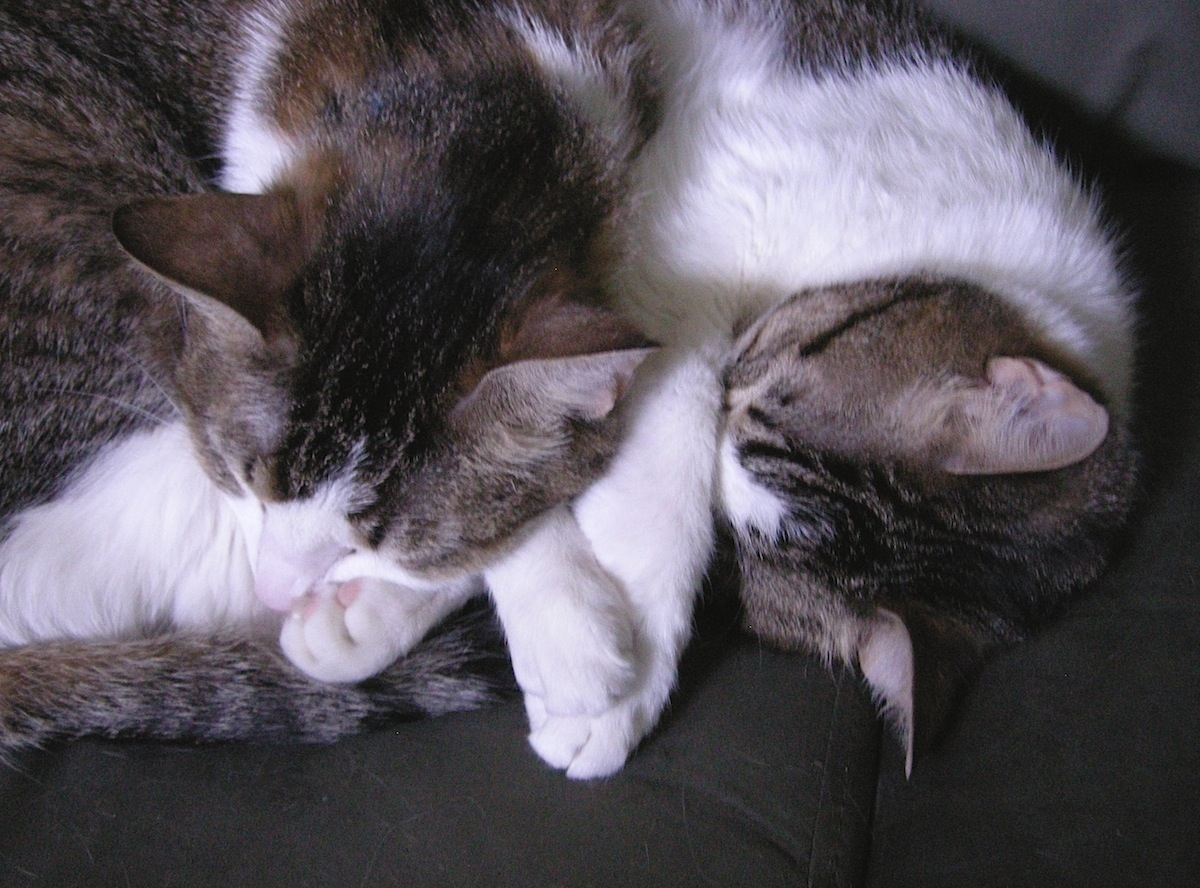
\includegraphics[width=5in]{./figures/kitties.jpg}
    \caption{This is a sample figure. Use .jpg, .pdf, or .png for best results.}
    \label{fig:sample-fig}
  \end{center}
\end{figure}

Figures are even easier. Figure \ref{fig:sample-fig}\footnote{Their
names are Bert and Ernie. Also, this is an example of how to make a footnote.} 
was produced using the following code:

\begin{verbatim}
  \begin{figure}[ht]
    \begin{center}
      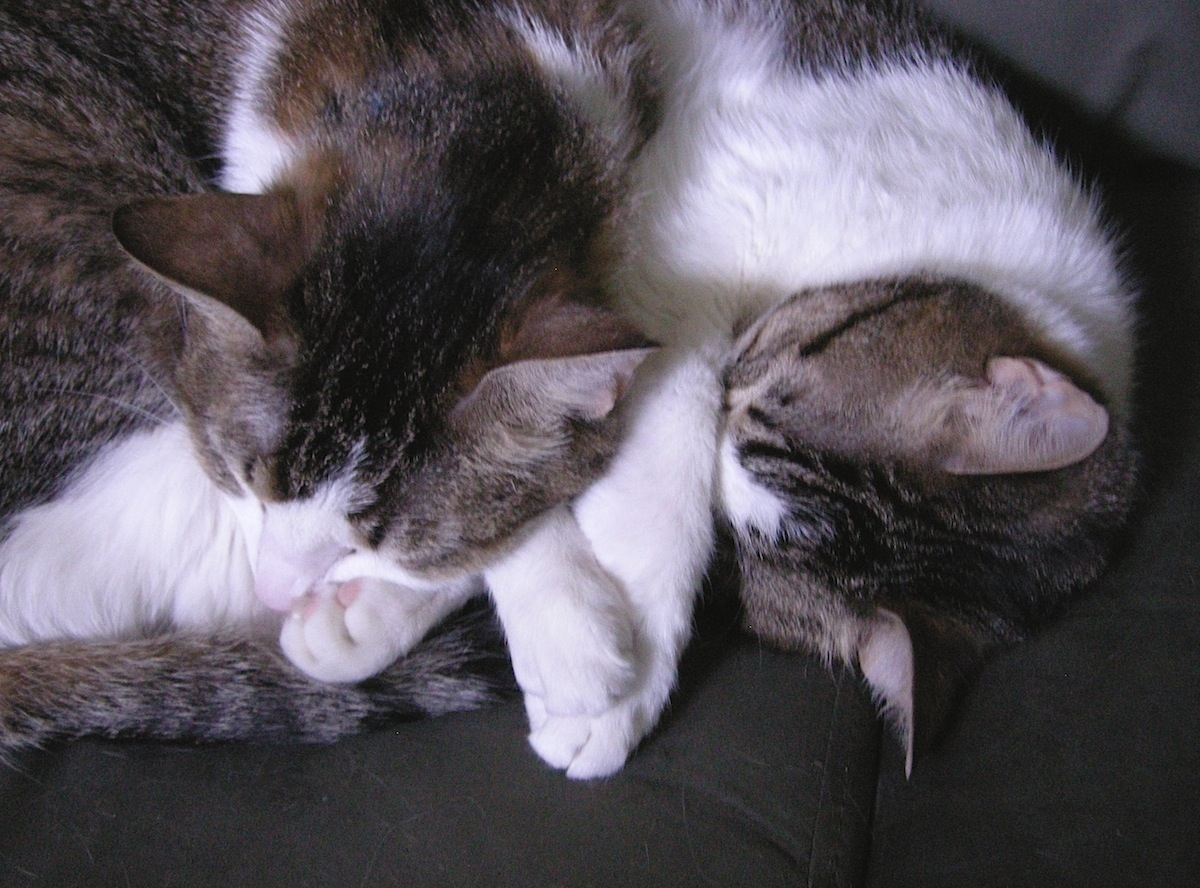
\includegraphics[width=5in]{./figures/kitties.jpg}
      \caption{This is a sample figure. Use .jpg, .pdf, or .png for best results.}
      \label{fig:sample-fig}
    \end{center}
  \end{figure}
\end{verbatim}
%
Again, we see code that centers the content and a label
immediately following the caption. \verb+\begin{figure}[ht]+ indicates that 
the figure
should go ``here'' (at that point in the code) or at the ``top'' of a page.
Sometimes \LaTeX ~won't put figures right where you want them, sometimes
for good reason. Other placement options can be found
readily with a little searching. Also, note that the command 
\verb+\includegraphics+ includes both instructions about where to find the
image and how large it should be in the document. Specifying the image size
requires the \verb+graphicx+ package. While it is a built-in package,
 you can see in the preamble that we still had to tell \LaTeX ~to use it.

\subsection{A Note on Special Characters}

As you've already seen, there are some characters that \LaTeX ~treats 
specially. Examples include the \% symbol (for comments), the \& symbol
(for tables) and the \_ and \$ symbols (used in mathematical notation).
If you want to use one of these symbols in your text, you will have to
``escape'' it using the $\backslash$ symbol. Other characters are a bit 
trickier, such as $\backslash$, which is generated using \verb+$\backslash$+.
The $\backslash$ character is not only for escaping special characters but
is also used at the beginning of \LaTeX ~macros and commands. Numerous examples
of this can be found by examining the {\tt .tex} files that generated this
document.
Improper use of special characters will either result in their not appearing
properly, unexpected formatting issues, or the document failing to compile.
There are many resources available discussing these issues. As a final note,
quotation marks are produced somewhat differently using the {\tt `} and {\tt '}
characters for opening and closing quotes respectively. For example, 
``quotation'' should be typed as {\tt ``quotation''}, {\it not} as 
{\tt "quotation"}. The latter yields "quotation", with improper quotes.

Additionally, you will find yourself having to do some additional work to
create letters and symbols that you don't find on your keyboard. Unlike
word processing software where special symbols and accented letters can usually
be produced by a combination of key presses (e.g. Ctrl+something+something),
in \LaTeX ~these symbols are created by special character sequences beginning
with $\backslash$. The mathematical symbol for inequality, $\neq$, is produced
with \verb+$\neq$+, and accented characters like \"o, \'o, and \^o are produced
using \verb+\"o, \'o,+ and \verb+\^o+.

\subsection{Citations and Cross-References}

The {\tt natbib} package is included here for handling references and
generating the bibliography. As with many other aspects of the document, you
have choices and there are many other style files and you may prefer to use
something else depending on formatting expectations for references
({\tt apacite} is likely a popular alternative for some). Different packages
have their own commands for handling references, so if you use
something other than {\tt natbib} you will have to attend to this, though
the similarities will likely outweigh the differences. With {\tt natbib},
you can use the \verb+\cite+ command to produce citations like 
\cite{baayen:2008}, with just the year in parentheses, or the \verb+\citep+
command to produce citations like \citep{gaylord:2013}, with the parentheses
enclosing both author and year. With parenthetical citations, you can also
include text before or after the reference by using square brackets
\citep[for example][and others]{kilgarriff:2004}. Multiple citations can be 
separated by commas, without spaces \citep{cruse:2000,klepousniotou:2008}. 
When using the non-parenthetical \verb+\cite+ command, references will still 
appear in parentheses if the authors' names are different.

References to examples, figures, tables, sections, etc is accomplished via the
\verb+\ref+ command, using the label you have included for the relevant item,
as in Example (\ref{ex:spaces}), Table \ref{tab:sample-table}, or Section
\ref{sec:content}. You can additionally use the \verb+\pageref+ command to
reference the page an item occurs on -- for example Table \ref{tab:sample-table}
is on page \pageref{tab:sample-table}.

\section{Typesetting Your Document}

If you're using a front end like MacTex, typesetting your document may be
just as easy as clicking a button. If you're doing it directly from the 
command line (for example, Terminal in OSX), it is just slightly more involved.
To produce a pdf of this document, with correct citations and cross-references,
you type 4 commands:

\begin{verbatim}
  pdflatex ut_thesis
  bibtex ut_thesis
  pdflatex ut_thesis
  pdflatex ut_thesis
\end{verbatim}
%
The first {\tt pdflatex} command generates the document and information 
about the citations and cross-references it contains. The {\tt bibtex} command 
gathers the necessary information from your {\tt .bib} file, and the two final
{\tt pdflatex} commands then properly generate the bibliography and
cross-referencing. If you haven't added any citations or cross-references,
a single {\tt pdflatex} may be all you need.

If you are a beginning user, you will likely opt for the easier route of doing
your document preparation entirely with the tools supplied by your \LaTeX
~distribution of choice, without needing to use the command line or other text
editors. This is fine. The advantages of the alternative route are more
applicable to more advanced users, and include the ability to generate other
document formats besides pdf (such as .ps and .dvi), and the familiarity of
using an editor one is already accustomed to. Ultimately, the choice is yours.

\section{Summary}
In this brief tutorial, we have covered a number of points. These include:

\begin{itemize}
  \item The anatomy of a \LaTeX ~project directory
  \item The structure of a .tex file, especially the preamble
  \item Numbered examples, tables, and figures
  \item Handling of special characters
  \item Citations and cross-references
  \item Typesetting
\end{itemize}
% Note how this commented line causes the following text not to be indented
This is enough to get started producing fairly substantial documents, and one
skill you will quickly gain is how to search for further information about
how to accomplish more nuanced goals. There's lots more -- for example, we
never even touched on one of \LaTeX's greatest strengths, which is the 
typesetting of mathematical formulas. There are also a great many packages to
allow you to typeset different types of charts and graphs. These are all
fairly straightforward though, and once you have them figured out, they are
generally quite easy to use. Good luck!
			     %% Input as separate file (recommended)

\chapter{Background}
\label{chap:background}
This chapter was included just to have another chapter, nothing to see here.


%% If you have appendices, uncomment the following line and include
%% your appendices the same way as chapters above.
\appendix

\chapter{Sample Appendix}
\label{chap:appendix}
This just exists to provide an example of an appendix

 
%% Force Bibliography to appear in contents                       
\addcontentsline {toc}{chapter}{Bibliography} 

%% Generate bibliography from your .bib file, in the style of your choice.
\bibliography{mybib}                    
\bibliographystyle{natbib}

%% Alternatively, comment out the two preceding lines and uncomment the two
%% following lines if you want to enter your bibliography items directly here.
% \begin{thebibliography}{..} 
% \end{thebibliography}                

%% Write your vita here; it can be anything allowed in in LaTeX2e par-mode.
%% Including a vita, which lists your permanent address, may be optional.
\begin{thesisauthorvita}                      
\end{thesisauthorvita}               

\end{document}                       %% Done.
